\documentclass{article} % For LaTeX2e
\usepackage{nips15submit_e,times}
\usepackage{hyperref}
\usepackage{url}
\usepackage{graphicx}
\usepackage{bbm}
\usepackage{amsmath}
\usepackage[psamsfonts]{amssymb}
\graphicspath{ {images/} }
\usepackage{algorithm}
\usepackage{algorithmic}

\usepackage[square,numbers]{natbib}
\bibliographystyle{unsrtnat}

%\documentstyle[nips14submit_09,times,art10]{article} % For LaTeX 2.09

\title{multi-region demixing of brain transcriptome}
% \addbibresource{nmf_multi.bib}

\author{
Lior Kirsch \\ Bar Ilan university \\ Ramat Gan 52900 Israel \\ 
\And
Gal Chechik \\ Bar Ilan university \\ Ramat Gan 52900 Israel \\
\texttt{gal.chechik@biu.ac.il} \\
}

\newcommand{\fix}{\marginpar{FIX}}
\newcommand{\new}{\marginpar{NEW}}
\newcommand{\reals}{\mathbb{R}}
\newcommand{\W}{W}
\renewcommand{\eqref}[1]{Eq.~(\ref{#1})}
\newcommand{\figref}[1]{Fig.~(\ref{#1})}
\newcommand{\figureref}[1]{Figure~(\ref{#1})}

%\nipsfinalcopy % Uncomment for camera-ready version

\begin{document}
\maketitle

\begin{abstract}
A nice abstract.
\end{abstract}

\section{Introduction}
\label{introduction}



Recent advances in molecular biology techniques allow to measure transcriptome profiles across the brain at unprecedented quality and price. Large datasets of gene expression in the brain are now available, covering  many brain regions, ages and species. RNA sequencing techniques now provides accurate genome-wide counts of transcripts for each gene and splice variant. Unfortunately however, when gene expression profiles is measured in a complex tissue, like the brain, the measured transcripts reflect an uncontrolled mix of expression from multiple cell types including neurons, astrocytes, oligodendrocytes and even blood and immune system cells. This limits the analysis and understanding that can be gained from transcriptome measures of the brain. While techniques have been developed to isolate and purify cells of individual types and measure their transcriptome. these techniques are costly and complex, and only a handful of cell-type isolated profiles have been collected so far. 

The current paper proposed a computational technique to demix brain transcriptome measurements. The idea is simple: when multiple samples are collected from the brain, their cellular composition often varies slightly from one sample to another. Each sample therefore reflects mixtures with different proportions of cell types. We propose here a model transcriptome profiles as a mixture, and describe how the latent component shared across samples can be found.

In the mouse brain, a demixing approach was recently applied to ISH transcriptome measures \cite{grange2014cell}, where expression profiles were demixed using known cell-type-specific profiles. Here we take a further step and apply blind demixing, inferring both the mixture components and their proportions. We use isolated cell types for validation but not during training. 

%Demixing transcriptome profiles into their components has been applied in various domains outside neuroscience \cite{}.

Importantly, collections of transcriptome measurements in the brain have a unique structure that we suggest to benefit from. In the brain, gene expression profile changes from one brain region to the other, in a way that often follows the developmental hierarchy of brain regions \cite{zapala2005}. This suggests that we can use a-priori knowledge about regions which are expected to share similar expression profiles. For instance, pyramidal cells can be found in most neocortex areas, hence may express a highly preserved set of genes. At the same time, neurons in the hippocampus an archeo-cortical region may exhibit a less similar expression profile.  Figure 1 shows a hierarchy of brain regions based on embryonic development. 

\begin{figure}[!hbt]
  \begin{minipage}[c]{0.65\textwidth}
    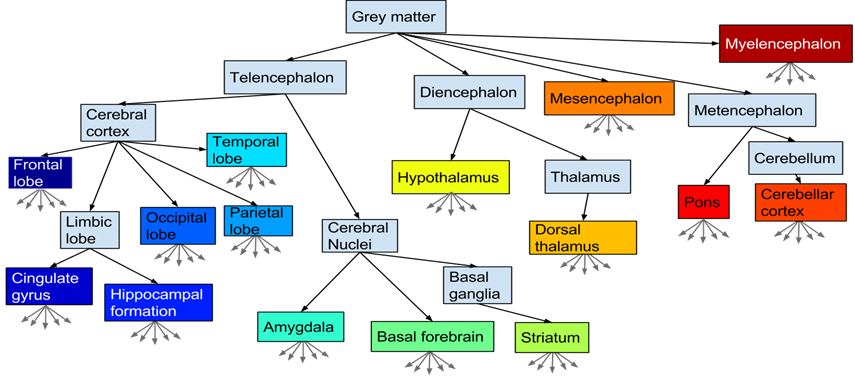
\includegraphics[width=\textwidth]{tree}
  \end{minipage}\hfill
  \begin{minipage}[c]{0.3\textwidth}
    \caption{Hierarchical relations among brain regions. An ontology of regions of the human brain has been created based on neural development. Colored boxes correspond to brain regions that we analyzed below. The color scheme is based on the embryonic origin of regions: red - hindbrain, blue - forebrain.} 
    \label{fig:bro}
  \end{minipage}
\end{figure}

This hierarchical structure suggests that when applying demixing to brainomics data, one should be careful not to treat all brain samples as homogeneously containing the same set of neurons and underlying expressed genes. Instead, we can take into account the relative similarity among brain structures. 

To combine the various sources of prior information, our approach is based on a probabilistic model with three components. First, a set of samples from a single brain regions is represented as a mixture of a smaller number of components. Second, we can include a prior on each of these underlying cell-type-specific profiles based on previous measurements. Third, we add pairwise attractive potentials, pushing expression profiles of related regions to be similar.
 
The paper is organized as follows: We start by describing a probabilistic model of expression mix, and describe the demixing optimization problem, and algorithms to solve it. We then describe the multi-region demixing problem, and an algorithm to solve it. In Section 4, we created a controlled mix data to evaluate the regime of parameters where the demixing algorithm works well. 


\section{A probabilistic model for demixing}

\newcommand{\x}{\mathbf{x}}
\renewcommand{\c}{\mathbf{h}}
\renewcommand{\H}{{H}}
\newcommand{\Htext}{{C}}
\newcommand{\paren}[1]{\left({#1}\right)}
\newcommand{\brackets}[1]{\left[{#1}\right]}
\newcommand{\norm}[1]{\|{#1}\|}
\newcommand{\argmin}{\operatornamewithlimits{argmin}}.

Our probabilistic model assumes that samples taken from the same brain region share common underlying factors, each factor reflecting the expression profile of an isolated cell type. The model also assumes that the expression profiles of different brain regions are similar but not identical, and therefore we aim to jointly learn all cell-type profiles of all regions. We start by describing a  probabilistic mixture model for samples from a \em{single} brain region, which we extend to the \em{multi-region} case in section 2.2.

\subsection{Model of a single brain region}
% ---------------------------------
Let $\{\x_1, \ldots, \x_n\} \in \reals^d$ be a set of samples. Our model assumes that each sample $\x_i$ is obtained from a noisy mixture of $K$ cell types, each having its own {\em {hidden profile}} $\{\c_1, \ldots \c_K \}\in \reals^d$.

We model each sample $x_i$ as a noisy mixture
\begin{equation*}
 \x_i = \sum_{k=1}^K p_{ik} \c_k + \xi_i \quad\forall i \quad,
\end{equation*}
where $p_{ik}$ is the proportion of the cell type $k$ in the sample $i$, $\sum_k p_{ik} = 1, \forall i$, and $\xi_i \sim N(0,\sigma^2)$ is additive Gaussian noise independent at each sample. We further assume a Gaussian prior distribution $p_0( \c_1, \ldots, \c_K)$ over each cell type $ \c_k  \sim N(\mu_k, \Sigma) $, and over the mixture proportions $p_0(p_1, \ldots p_K)$. The parameters $\mu_k$ and $\Sigma$ can be estimated in advance from available measurements of expression in isolated cell types \cite{okaty2011cell,darmanis2015survey}.

Together, the probability of an observed sample $x_i$ is
\begin{equation*}
    P(\x_1,\ldots,\x_n | \{\c_k\}, \{p_{ik}\}) =  \frac{1}{\sqrt{2\pi}\sigma} \exp\left(-\frac{1}{2\sigma} (x_i - \sum_{k=1}^K p_{ik} \c_k)^2 \right)
\end{equation*}
and the minus log posterior of all the data equals (up to linear constants)
\begin{equation*}
    - log P(\x_1,\ldots,\x_n, \H, P| \mu, \Sigma) \propto
    \sum_{i=1}^n \paren{ \frac{1}{\sigma} (x_i - \sum_{k=1}^K p_{ik} \c_k)^2 }
     + \sum_{k=1}^K (c_k-\mu_k)^T\Sigma^{-1}(c_k-\mu_k)
\end{equation*}

Using matrix notation, we denote by $\H$ the $K \times d$ matrix of hidden profiles per cell type whose columns are $\brackets{\c_1, \ldots, \c_K}$; we denote by $W$ the $n \times K$ matrix of proportions $p_{ik}$,
and by $X$ the matrix whose columns are the samples $\brackets{\x_1,..., \x_n}$. This yields that maximizing the log posterior is equivalent to minimizing 
\begin{equation}
    \label{eq-single}
    \begin{aligned}
        & \underset{\cal{\H},\cal{W}}{\text{min}}  
        & & \norm{X - W \H}_F^2 + \sigma \norm{ \H - M }^2_{(\Sigma^{-1})}\\
            & \text{subject to} &
            & W^r_{l,j} \geq 0 \;\; \forall j, l, \\
        & & & H^r_{j,d} \geq 0 \;\;\forall j, d \\
        & & & \sum_j W^i_{l,j} = 1 \;\; \forall l \\
        \end{aligned}
\end{equation}
where $\norm{\cdot}_F$ is the Frobenius norm, $M$ is a matrix whose columns are the expected cell-type profiles $\mu_k$ and  $\|\cdot\|_{\Sigma}$ is the norm through a PSD matrix $\Sigma$. The constraints on $\W$ are because the elements in each row of $\W$ are mixture probabilities. The constraints on $\H$ are because the elements of $\H$ are counts of expressed transcripts.

\subsection{Multiple regions}
%-------------------------------
We now turn to extend single-region demixing to handle demixing of samples collected from several brain regions. 
As far as we are aware, this is the first probabilistic model for demixing multiple sets of samples.

We assume that expression profiles of an each cell type can vary from one region to another, but is likely to remain similar. The strength of similarity between the expression profiles in two regions depends on how closely related two brain regions are. For instance, neurons in cortical regions may be very similar to each other, less similar to the hippocampal neurons and far less similar to the cerebellar neurons. 

To capture these relations our model introduces pair-wise attractive potentials between the cell-type profile in one region $\c^r_k$ to the profile of the same cell type in another region $\c^s_k$. The strength of the attraction depends on the relatedness $\phi_{r,s}$ of two brain regions, and on a global hyper parameter that controls the relative weight of edge potentials compared with node potentials. Together, this yields pairwise potential terms of the form 
$\lambda \phi_{r,s}|| \c^r_k - \c^s_k||^2$.

This soft-sharing approach can be seen as a balance between two extremes. At one extreme (no pairwise attraction, $\lambda=0$), demixing of each regions is trained independently. With current datasets, this approach usually has too few samples per regions.  At the other extreme (strong pairwise attraction, $\lambda \gg 0$), one could treat all samples as being created from a single set of underlying latent factors, as if all brain regions share a single expression profiles per cell-type. In this case, more samples are available for estimating the (fewer) latent factors, but the wrong assumes that expression is homogeneous across the brain   distorts the resulting profiles. Our soft-sharing approach bridges the two extremes by controlling how profiles of different regions share common traits. Similar soft sharing has often been used in supervised multi-task learning (MTL). 

Formally, given sets of samples from $R$ regions ${\cal{X}} = \{X^1,\ldots, X^R\}$, where $X^r = \{\x^r_1, \ldots, \x^r_{n_r} \}$, we learn $R$ sets of hidden cell-type-specific profiles ${\cal{\H}} = \{\H^1,\ldots, \H^R\}$ and their corresponding proportions ${\cal{W}} = \{ W^1,\ldots W^R\}$. Adding Gaussian potentials over cell-type profiles from a pair of regions ($\H^r$, $\H^s$) with a weight of $\lambda_{r,s}$ amounts to a quadratic term in the log posterior. This therefore yields the following optimization problem
\begin{equation}
    \label{eq-multi}
    \begin{aligned}
        & \underset{\cal{\H},\cal{W}}{\text{min}}  
        & & \sum_{r=1}^R  \| X^r - W^r \H^r \|_F^2
        + \sum_{r=1}^R  \sigma^r \| M^r - \H^r \|^2_{(\Sigma^{-1})}  
        + \sum_{r \neq s} \lambda \phi_{r , s} \| \H^r - \H^s \|_F^2  \\
        & \text{subject to} &
            & W^r_{l,j} \geq 0 \;\; \forall j, l, r\\
        & & & H^r_{j,d} \geq 0 \;\;\forall j, d, r \\
        & & & \sum_j W^r_{l,j} = 1 \;\; \forall l,r \;. 
    \end{aligned}
\end{equation}
Once again the constraints on $\W$ are since these are the mixture proportions, and the constraints on all $\H$ reflecrt the fact that $\H$ holds counts of transcripts.

The proposed model is interestingly related to Markov random fields (MRFs). Consider a case where the mixture proportions $\cal{W}$ are given, then the probabilistic model over $\cal{\H}$ can be viewed as an MRF, where nodes correspond to the profiles of individual cell types across all regions $\c^1_1,\ldots, \c^r_k, \ldots \c^R_K$, node potentials reflect the priors $p_0(\c_k)$ based on known expression of individual cell types at various regions, and edge potentials reflect region-to-region similarity terms $\lambda \phi_{r,s}|| \c^r_k - \c^s_k||^2$. 

The next section discusses the algorithms we use to optimize this objective.

\section{Optimization}
% =====================
We now describe algorithms for optimizing the multi-region problem of \eqref{eq-multi}. We start with reviewing existing approaches for single-region demixing and then discuss multi-region demixing. 


% Our problem is well suited for performing block coordinate descent, both on the profiles and proportion matrices and both on the regions. At each iteration, we update the set of coordinates of a single region and freeze the coordinate of the rest of the region. After we update the profile matrices $H_n$ we proceed to update its proportion matrix $W_n$. Then, we cycle through the rest of the region and repeat until we converge. 

\subsection{Single-region demixing}
The demixing problem of \eqref{eq-single} is separately convex in $\H$ and $\W$ (quadratic objective with linear constraints), but not jointly convex in both. When the prior is discarded, it becomes equivalent to non-negative matrix factorization (NMF) \cite{leenmfs}, which has been intensively studied. Several approaches have been proposed to minimize the NMF objective.
%
% For the convergence I think we can claim something similar to:
% http://bioinformatics.oxfordjournals.org/content/23/12/1495.full
% In the section:
% Convergence properties of sparse NMF algorithms
% http://www.sciencedirect.com/science/article/pii/S0167637799000747#
Here we tested four methods: Multiplicative updates (MU) \cite{leenmfs}, and three variants of alternative least square (ALS) \cite{lin2007projected,kim2008activeset,kim2011fast}. 

{\bf {Multiplicative updates (MU)}}. Lee and Seung \cite{leenmfs} described an NMF algorithm based on multiplicative updates of W and \Htext. At each step, each coordinate of \Htext (and \W) is multiplied by a non-negative scalar, which gaurantees that non-negativity is maintained: $H_{qj} \leftarrow H_{qj} \frac{(W^TX)_{qj}}{((W^TW)H)_{qj}} \quad
\forall 1\leq q \leq k, 1\leq j \leq n$ and $W_{iq} \leftarrow W_{iq} \frac{(XH^T)_{iq}}{(W(HH^T))_{iq}} \quad \forall 1\leq i \leq m, 1\leq q \leq k$.
This procedure is guaranteed to converge \cite{leenmfs,lin2007convergence}. 
% They showed the objective after these updates is %non-increasing. Although in practice the %muliplcative-update method works well, it was suggest %by Gonzalez and Yin Zhang %\cite{gonzalez2005accelerating}  that the %non-increasing updates may not converge to a %stationary point within realistic time.

{\bf{Alternating least squares} (ALS)} A second set of approaches to minimize the NMF objective is based on the fact that the optimization problem in \eqref{eq-single} is convex in each of the variables \W (or \Htext), hence one can iterate between efficiently updating $\W$ and updating $\H$. This approach can be viewed as a block-coordinate minimization approach. In ALS, the two matrices are  repeatedly updated using $ W^{t+1} = \argmin_{W \geq 0 } f(W^t, H^t)$ and $H^{t+1} = \argmin_{H \geq 0 } f(W^{t+1},H^t)$. Several different method of solving non negative least squares (NNLS) have been proposed some especially tuned for NMF. \citet{lin2007projected} proposed projected gradient decent with step that is chosen using the Armijo rule. 
Kim and park \cite{kim2008activeset,kim2011fast} use an active set method to solve NNLS. They group their variables to an active set and a passive set and 
exchange variables between the two to find the optimal sets. Variables are added to the passive set (the set of strictly positive variables) if they improve the score. Notice that if the passive set was known in advance, then an NNLS problem is a simple unconstrained least squares. Another variant of this concept is done by the "the block pivoting method" which allows to change multiple variable between groups per iteration (as appose to a single variable using the active set method) \cite{kim2011fast}. {\bf{THE ALS SECTION SHOULD BE MUCH SHORTER}}

In \eqref{eq-single} the rows of $\W$ are constrained to sum to one. This constraint is often relaxed during optimization. In practice, it is often replaced with a simple heuristic of normalizing each row of W after the optimization is completed. 

The above discussion focused on the first term in \eqref{eq-single}, omitting the prior term. Using the fact that we alternate between $\W$ and $\H$ the priors can be elegantly added by a simple transformation. Each time before we solve the minimization problem for H we perform:
$ X_{priors} = \Big[ X ;\Sigma^{-\frac{1}{2}} \Big]  $  ,  $ \W_{priors} = \Big[  \W ; \Sigma^{-\frac{1}{2}} M \Big]  $. We then find the minimum for $H$ using $X_{priors} $ and $W_{priors} $. 



\subsection{Multi-region demixing}
% ----------------------------------
The multi-region demixing model of \eqref{eq-multi} defines a jount optimization problem over all cell-type profiles $\cal{\H}$ and their proportions across all regions $\cal{\W}$.

Given values for the hyper parameters $\lambda$, $\sigma^r$ and $\phi_{r,s}$, 
we optimize \eqref{eq-multi} by extending the alternating least square (ALS) approach, this time solving separately for ${\H^r}$ and ${\W^r}$ of each region given all the other regions. This approach has similar convergence guarantees as the original ALS approach.  {\bf{ LIOR CAN YOU SPECIFY? AND ADD A REF}}

We initialize $\W^r$ with values in the range [0,1] and initialize $\H^r$ by random data samples with multiplicative noise. In practice, we found that it helped to start optimization by solving for each region separately, alternating over $\H$ and $\W$ for that region. We believe that this helped the profiles to more easily reconstruct their own unique profile. This 'warm-start' was then used to initialize the global ALS optimization. 
% We have also experimented with a few method to enforce the constrains on the proportion matrix. while some s%%Then prior to starting the loop, we warm initialize the profiles by performing a single step of block coordinate decent for each ($H^r,W^r$).

The values of the hyper parameters $\lambda$ and $\sigma^r$ can be found using cross validation. However, searching over all pairwise weights $\phi_{r,s}$ maybe prohibitive. We therefore used prior knowledge to determine the values of $\phi_{r,s}$. The strength of these hyper parameters reflects our prior belief on how strongly cell-type specific expression should be similar in two given regions, like the the expected similarity of a cortical to a hippocampal neuron.
To determine the values of $\phi_{r,s}$, we used a brain region hierarchy developed by the Allen institute of brain research (\figref{fig:bro}) to compute the tree-depth of the closest common ancestor of two brain regions $r$ and $s$. We used this depth as an estimate of $\log(\phi_{r,s})$. For example, the cerebellum and the occipital lobe  in this hierarchy are joined only at the root so we set their $\phi_{cerebellum, occipital} = \exp(1)$. 
%Specifically, at stage $t+1$ we update the profile matrix of %region r$ \H_r^{t+1} $ using the related profiles as priors.
%For the regularize parameters we use a base $\lambda$ times a distance factor between pairs of regions. 

Algorithm (1) desribes our training procedure.

\begin{algorithm}[tbh]
   \caption{Multi-region demixing}
   \label{alg:multimix}
   \begin{algorithmic}[1]
   \STATE {\bfseries input:} training data $X$, number of steps, $\lambda$, $\{\sigma^r\}$, $\{\phi_{r,s}\}$, $\{\mu^r_k\}$, $\Sigma$
   \STATE {\bfseries initialize:} for every region $r$
   \STATE \quad Initialize $\W^r$ and $\H^r$ with random values.
   %\REPEAT
   \STATE {\bfseries warm-start:} for every region $r$ 
   \STATE \quad Find optimal $\W^r$ and $\H^r$ for the single-region objective \eqref{eq-single}
   \STATE \quad $H^r = \argmin_{H \geq 0 } \| X^r - W^rH\|^2_F +  \sigma^r \| M^r - \H \|^2_{(\Sigma^{-1})} $
   \STATE \quad $ W^r = \argmin_{W \geq 0} \| X^r - WH^r\|^2_F $
   \REPEAT
   \STATE Select a region $r$ from a predefined random permutation.
   \STATE Find optimal $\W^r$ and $\H^r$ for the multi-region objective \eqref{eq-multi} using the rest of the regions as priors.
   \STATE  $H^r = \argmin_{H \geq 0 } \| X^r - W^rH\|^2_F + \sum_{r \neq s} \lambda \phi_{r , s} \| \H - \H^s \|_F^2  + \sigma^r \| M^r - \H \|^2_{(\Sigma^{-1})} $
   \STATE  $ W^r = \argmin_{W \geq 0} \| X^r - WH^r\|^2_F $
   \UNTIL{stopping condition}
\end{algorithmic}
\end{algorithm}




\section{Related methods}
Demixing of transcriptome measurements into cell-type specific profiles has been mostly applied when a set of ground-truth underlying factors is known. \citet{shen2010cell} described demixing of 
whole-blood gene expression datasets from kidney transplants. \citet{grange2014cell} used isolated profiles of neurons and glia \cite{okaty2011cell} to map cell-type proportions across ISH measures of the mouse brain.

{\bf {ADD refs to blind demixing in immunology}}

Joint non negative matrix factorization of several matrices has been previously studied by \citet{lee2009group}. Their formulation introduced  both attractive and repulsive pairwise potentials, optimized using multiplicative updates. A Bayesian group factorization model was presented in \citet{shin2012bayesian}. Somewhat related, is the work by \citet{wang2012group}, who studied matrix factorization where some factors are shared across matrices.






\section{Controlled experiments}

\label{Synthetic_exp}


With the goal of comparing optimization methods and finding the regime of hyper parameters where multi-region demixing is beneficial, we start with a series of experiment on controlled data where the latent factors are known and used as a ground truth. We first describe how the dataset was created and then characterize how performance depends on the number of samples and the number of latent factors (cell types).


\subsubsection*{Creating the mixture dataset}
We created controlled mixtures from a set of real transcriptome measurements, collected from isolated cells



We gathered profiles for the 3 population of cell types in the brain: neurons, astrocytes and oligodendrocytes. Each profile is represented by 14580 genes. The cell type profiles were extracted from 7 brain regions:  cortex layer 5A, cortex layer 5B, cortex layer 6, striatum, cerebellum, brainstem and the spinal cord \cite{okaty2011cell}. For each region, we mixed the profiles using ratio taken from the literature \cite{Herculano2014}. cortical regions ( 0.7; 0.1;0.2) , cerebellum (0.5; 0.15; 0.35) , other (0.65;  0.1;0.25)  (neuron, astrocytes, oligodendrocytes).

We have added variability to the proportions of the samples by multiplying them by random value [0,1] and scaling back so that they sum to 1.
Finally, we introduced noise for each sample by multiplying it with by a normal random variable with unit mean. We insure that the normally distributed number is positive.

We evaluated the reconstructed profiles by computing their spearman correlation with the true profiles. We then, matched the best true profiles to the reconstructed profiles.

Each time we sampled n noisy samples and reconstructed the profiles using these samples. The error bars in figure  represented the sem over 30 repetitions.  

{\bf{Move to the experiments section? Also fix the 1st sentence}} Since NMF is a non-convex problem bench-marked a couple of methods on our problem. We wanted to test if when initialized using the same starting points they will perform differently. We tested 4 optimization techniques and found that all performed better with more samples. When the number of sample is sufficiently large we did not observe much difference in the performance of the different methods. while in a small number of samples the block-pivoting and the active-set performed slightly better (both had the same level of performance) Figure \ref{fig:controlled_exp}.

\subsubsection*{analyzing number of samples}
We notice that in the regime of limited samples there is sweet spot where we benefit from using regularization over the naive cases. As we increase the number of samples the benefit that we gain by using our method diminishes Figure \label{fig:controlled_exp}(b). With enough samples we solving the individual problems performs almost just as well. 



\begin{figure}[!hbt]
   (a) \hspace{120pt}(b) \hspace{120pt}(c) \hspace{120pt}
   \centering
     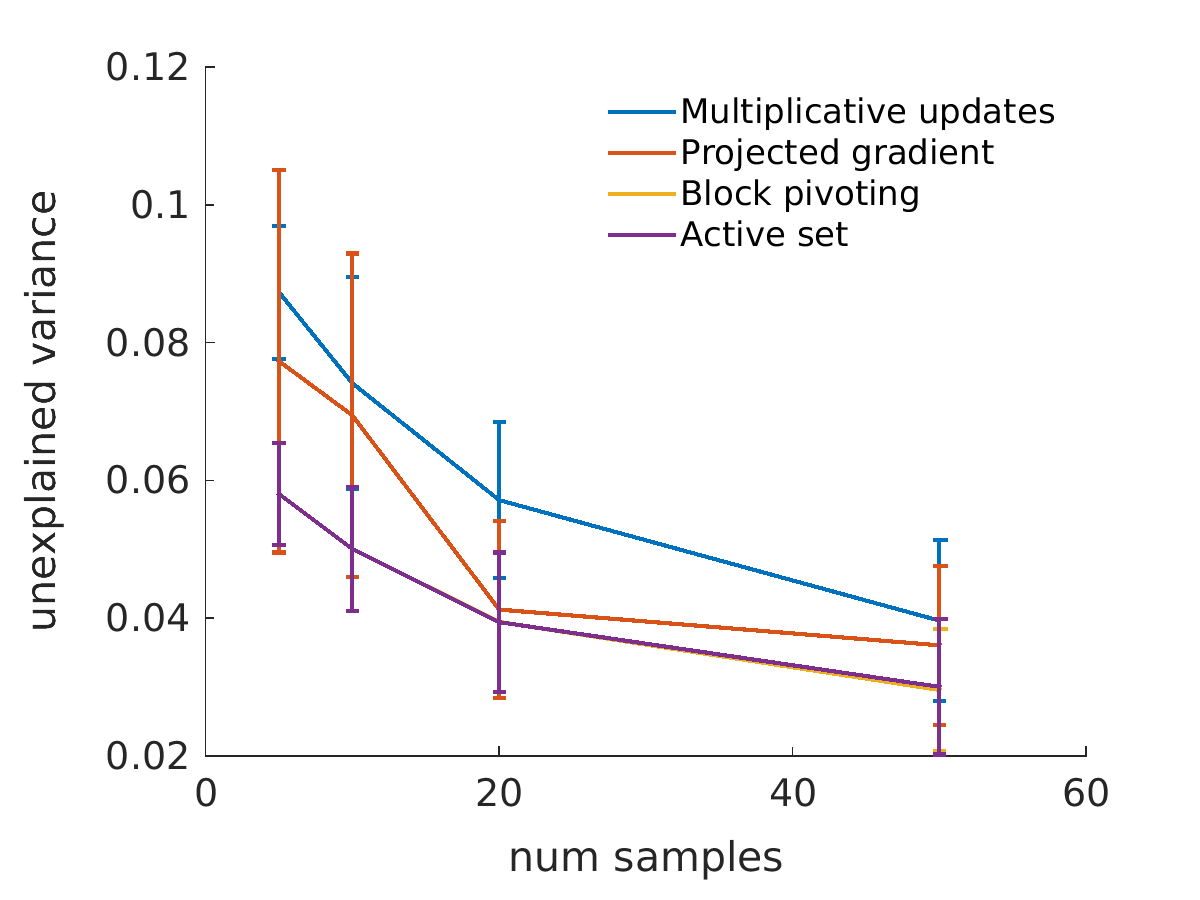
\includegraphics[width=0.32\textwidth]{methods}
     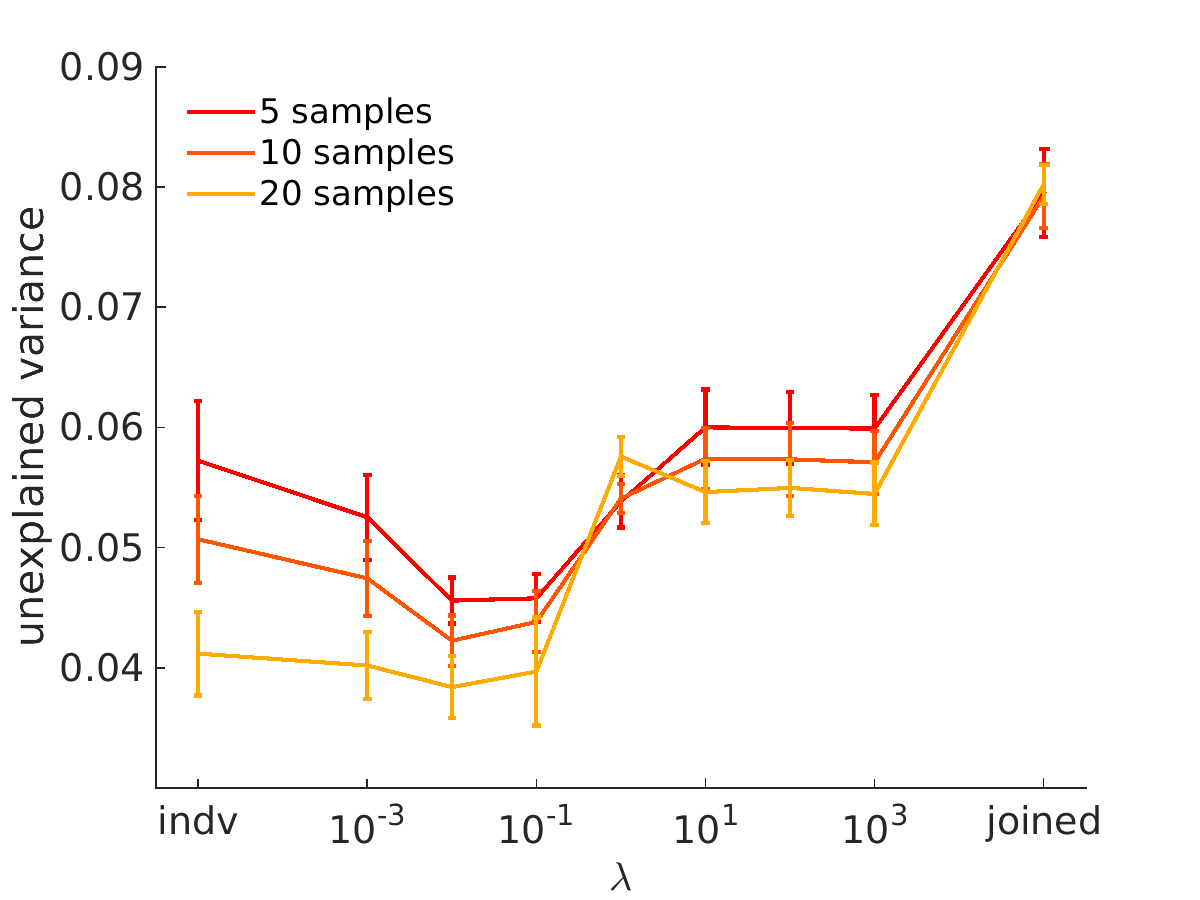
\includegraphics[width=0.32\textwidth]{lambda_sample_with20}
     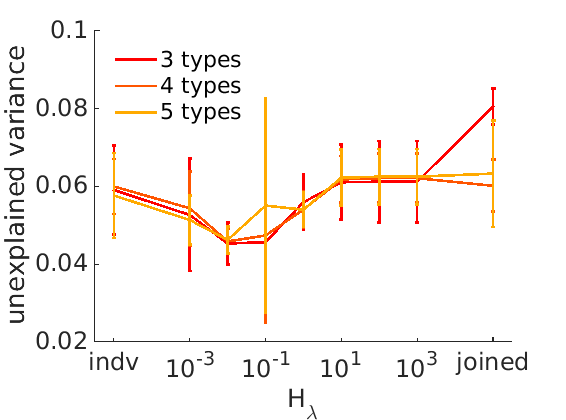
\includegraphics[width=0.32\textwidth]{num_types}
    \caption{The effect of $\lambda$ on reconstruction}, 
    (a)  With a single region, all optimization method perform better as we introduced more samples. With a limited number of samples the active set and the block pivoting approaches performed the best. (b) Using multiple regions, the regularized connection between the region profiles help to reconstruct the original profiles. This is especially noticeable when only few samples are available for each region. (c) ????
    \label{fig:controlled_exp}
\end{figure}




\subsubsection*{analyzing number of cell types}

As we increase the number of types the we are able to numerically better reconstruct the data matrix because we are allowing an approximation with of a larger rank. The reconstructed was able to recover the original profiles and to provide other vectors. Overall it seems that this coincide with Ockham's razor and we can select simplest model which still capture the data. 





\section{Human brain data}
\label{Human_exp}




Human tissues are not easy to come by and 
We are interested in demixng RNA sequencing data (RNA-seq) that waseperating tissues
Unfortunately, there is no dataset that measure single cell profiles in the human brain. This posses a great challenge but also a great opportunity for blind-demixng. 
We use the brainspan dataset \cite{brainspan} to 
NMF since it is clear that using single cell profiles the profiles


We used brainspan data from K different region which was gathered from 8 humans subjects (we limit our anaylsis only to adult humans older than 17). There are ~8 samples from each region. Each expression is represtented by a vector of 52376 which hold sequnacing data both for coding region in the DNA and for noncoding regions. 

To evaluate the data we computed correlation between the reconstructed profiles and t
About the data




\begin{figure}[!hbt]
   (a) \hspace{120pt}(b) \hspace{120pt}(c) \hspace{120pt}
   \centering
     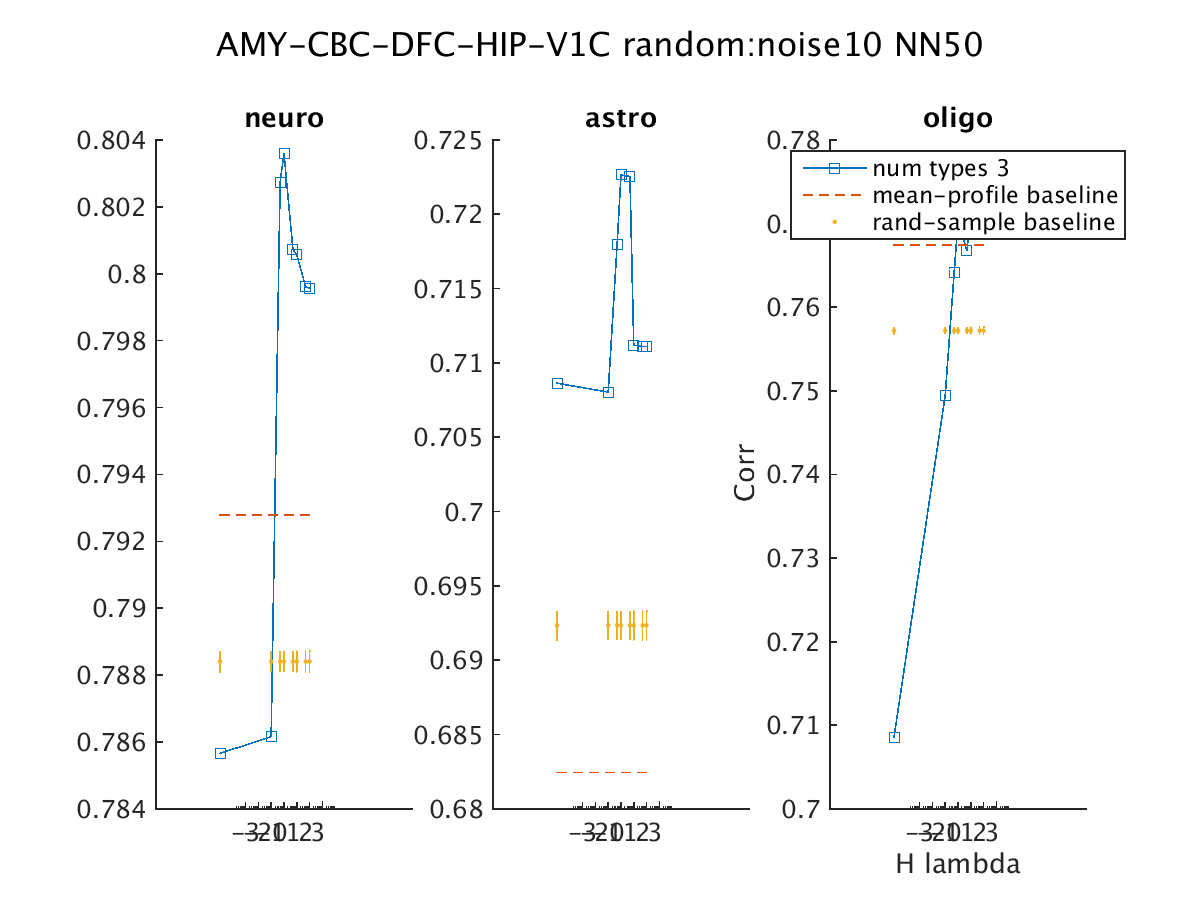
\includegraphics[width=0.95\textwidth]{human_data}
     caption{The effect of $\lambda$ on reconstruction}, 
    (a)  With a single region, all optimization method perform better as we introduced more samples. With a limited number of samples the active set and the block pivoting approaches performed the best. (b) Using multiple regions, the regularized connection between the region profiles help to reconstruct the original profiles. This is especially noticeable when only few samples are available for each region. (c) ????
    \label{fig:controlled_exp}
\end{figure}





[Add in the human experiment section We first verified that the brain regions in our data agree with the dev ontology: we clustered the brain regions in a hierarchical way and compared the resulting hierarchy to the dev ontology. We obtained very strong agreement …]. 


\section{Summary}




\bibliography{nmf_multi}

\end{document}


\subsection{Retrieval of style files}

The style files for NIPS and other conference information are available on the World Wide Web at
\begin{center}
   \url{http://www.nips.cc/}
\end{center}
The file \verb+nips2015.pdf+ contains these 
instructions and illustrates the
various formatting requirements your NIPS paper must satisfy. \LaTeX{}
users can choose between two style files:
\verb+nips15submit_09.sty+ (to be used with \LaTeX{} version 2.09) and
\verb+nips15submit_e.sty+ (to be used with \LaTeX{}2e). The file
\verb+nips2015.tex+ may be used as a ``shell'' for writing your paper. All you
have to do is replace the author, title, abstract, and text of the paper with
your own. The file
\verb+nips2015.rtf+ is provided as a shell for MS Word users.

The formatting instructions contained in these style files are summarized in
sections \ref{gen_inst}, \ref{headings}, and \ref{others} below.

%% \subsection{Keywords for paper submission}
%% Your NIPS paper can be submitted with any of the following keywords (more than one keyword is possible for each paper):

%% \begin{verbatim}
%% Bioinformatics
%% Biological Vision
%% Brain Imaging and Brain Computer Interfacing
%% Clustering
%% Cognitive Science
%% Control and Reinforcement Learning
%% Dimensionality Reduction and Manifolds
%% Feature Selection
%% Gaussian Processes
%% Graphical Models
%% Hardware Technologies
%% Kernels
%% Learning Theory
%% Machine Vision
%% Margins and Boosting
%% Neural Networks
%% Neuroscience
%% Other Algorithms and Architectures
%% Other Applications
%% Semi-supervised Learning
%% Speech and Signal Processing
%% Text and Language Applications

%% \end{verbatim}




First level headings are lower case (except for first word and proper nouns),
flush left, bold and in point size 12. One line space before the first level
heading and 1/2~line space after the first level heading.

\subsection{Headings: second level}

Second level headings are lower case (except for first word and proper nouns),
flush left, bold and in point size 10. One line space before the second level
heading and 1/2~line space after the second level heading.

\subsubsection{Headings: third level}

Third level headings are lower case (except for first word and proper nouns),
flush left, bold and in point size 10. One line space before the third level
heading and 1/2~line space after the third level heading.

\section{Citations, figures, tables, references}
\label{others}

These instructions apply to everyone, regardless of the formatter being used.

\subsection{Citations within the text}

Citations within the text should be numbered consecutively. The corresponding
number is to appear enclosed in square brackets, such as [1] or [2]-[5]. The
corresponding references are to be listed in the same order at the end of the
paper, in the \textbf{References} section. (Note: the standard
\textsc{Bib\TeX} style \texttt{unsrt} produces this.) As to the format of the
references themselves, any style is acceptable as long as it is used
consistently.

As submission is double blind, refer to your own published work in the 
third person. That is, use ``In the previous work of Jones et al.\ [4]'',
not ``In our previous work [4]''. If you cite your other papers that
are not widely available (e.g.\ a journal paper under review), use
anonymous author names in the citation, e.g.\ an author of the
form ``A.\ Anonymous''. 


\subsection{Footnotes}

Indicate footnotes with a number\footnote{Sample of the first footnote} in the
text. Place the footnotes at the bottom of the page on which they appear.
Precede the footnote with a horizontal rule of 2~inches
(12~picas).\footnote{Sample of the second footnote}

\subsection{Figures}

All artwork must be neat, clean, and legible. Lines should be dark
enough for purposes of reproduction; art work should not be
hand-drawn. The figure number and caption always appear after the
figure. Place one line space before the figure caption, and one line
space after the figure. The figure caption is lower case (except for
first word and proper nouns); figures are numbered consecutively.

Make sure the figure caption does not get separated from the figure.
Leave sufficient space to avoid splitting the figure and figure caption.

You may use color figures. 
However, it is best for the
figure captions and the paper body to make sense if the paper is printed
either in black/white or in color.
\begin{figure}[h]
\begin{center}
%\framebox[4.0in]{$\;$}
\fbox{\rule[-.5cm]{0cm}{4cm} \rule[-.5cm]{4cm}{0cm}}
\end{center}
\caption{Sample figure caption.}
\end{figure}

\subsection{Tables}

All tables must be centered, neat, clean and legible. Do not use hand-drawn
tables. The table number and title always appear before the table. See
Table~\ref{sample-table}.

Place one line space before the table title, one line space after the table
title, and one line space after the table. The table title must be lower case
(except for first word and proper nouns); tables are numbered consecutively.

\begin{table}[t]
\caption{Sample table title}
\label{sample-table}
\begin{center}
\begin{tabular}{ll}
\multicolumn{1}{c}{\bf PART}  &\multicolumn{1}{c}{\bf DESCRIPTION}
\\ \hline \\
Dendrite         &Input terminal \\
Axon             &Output terminal \\
Soma             &Cell body (contains cell nucleus) \\
\end{tabular}
\end{center}
\end{table}

\section{Final instructions}
Do not change any aspects of the formatting parameters in the style files.
In particular, do not modify the width or length of the rectangle the text
should fit into, and do not change font sizes (except perhaps in the
\textbf{References} section; see below). Please note that pages should be
numbered.

\section{Preparing PostScript or PDF files}

Please prepare PostScript or PDF files with paper size ``US Letter'', and
not, for example, ``A4''. The -t
letter option on dvips will produce US Letter files.

Fonts were the main cause of problems in the past years. Your PDF file must
only contain Type 1 or Embedded TrueType fonts. Here are a few instructions
to achieve this.

\begin{itemize}

\item You can check which fonts a PDF files uses.  In Acrobat Reader,
select the menu Files$>$Document Properties$>$Fonts and select Show All Fonts. You can
also use the program \verb+pdffonts+ which comes with \verb+xpdf+ and is
available out-of-the-box on most Linux machines.

\item The IEEE has recommendations for generating PDF files whose fonts
are also acceptable for NIPS. Please see
\url{http://www.emfield.org/icuwb2010/downloads/IEEE-PDF-SpecV32.pdf}

\item LaTeX users:

\begin{itemize}

\item Consider directly generating PDF files using \verb+pdflatex+
(especially if you are a MiKTeX user). 
PDF figures must be substituted for EPS figures, however.

\item Otherwise, please generate your PostScript and PDF files with the following commands:
\begin{verbatim} 
dvips mypaper.dvi -t letter -Ppdf -G0 -o mypaper.ps
ps2pdf mypaper.ps mypaper.pdf
\end{verbatim}

Check that the PDF files only contains Type 1 fonts. 
%For the final version, please send us both the Postscript file and
%the PDF file. 

\item xfig "patterned" shapes are implemented with 
bitmap fonts.  Use "solid" shapes instead. 
\item The \verb+\bbold+ package almost always uses bitmap
fonts.  You can try the equivalent AMS Fonts with command
\begin{verbatim}
\usepackage[psamsfonts]{amssymb}
\end{verbatim}
 or use the following workaround for reals, natural and complex: 
\begin{verbatim}
\newcommand{\RR}{I\!\!R} %real numbers
\newcommand{\Nat}{I\!\!N} %natural numbers 
\newcommand{\CC}{I\!\!\!\!C} %complex numbers
\end{verbatim}

\item Sometimes the problematic fonts are used in figures
included in LaTeX files. The ghostscript program \verb+eps2eps+ is the simplest
way to clean such figures. For black and white figures, slightly better
results can be achieved with program \verb+potrace+.
\end{itemize}
\item MSWord and Windows users (via PDF file):
\begin{itemize}
\item Install the Microsoft Save as PDF Office 2007 Add-in from
\url{http://www.microsoft.com/downloads/details.aspx?displaylang=en\&familyid=4d951911-3e7e-4ae6-b059-a2e79ed87041}
\item Select ``Save or Publish to PDF'' from the Office or File menu
\end{itemize}
\item MSWord and Mac OS X users (via PDF file):
\begin{itemize}
\item From the print menu, click the PDF drop-down box, and select ``Save
as PDF...''
\end{itemize}
\item MSWord and Windows users (via PS file):
\begin{itemize}
\item To create a new printer
on your computer, install the AdobePS printer driver and the Adobe Distiller PPD file from
\url{http://www.adobe.com/support/downloads/detail.jsp?ftpID=204} {\it Note:} You must reboot your PC after installing the
AdobePS driver for it to take effect.
\item To produce the ps file, select ``Print'' from the MS app, choose
the installed AdobePS printer, click on ``Properties'', click on ``Advanced.''
\item Set ``TrueType Font'' to be ``Download as Softfont''
\item Open the ``PostScript Options'' folder
\item Select ``PostScript Output Option'' to be ``Optimize for Portability''
\item Select ``TrueType Font Download Option'' to be ``Outline''
\item Select ``Send PostScript Error Handler'' to be ``No''
\item Click ``OK'' three times, print your file.
\item Now, use Adobe Acrobat Distiller or ps2pdf to create a PDF file from
the PS file. In Acrobat, check the option ``Embed all fonts'' if
applicable.
\end{itemize}

\end{itemize}
If your file contains Type 3 fonts or non embedded TrueType fonts, we will
ask you to fix it. 

\subsection{Margins in LaTeX}
 
Most of the margin problems come from figures positioned by hand using
\verb+\special+ or other commands. We suggest using the command
\verb+\includegraphics+
from the graphicx package. Always specify the figure width as a multiple of
the line width as in the example below using .eps graphics
\begin{verbatim}
   \usepackage[dvips]{graphicx} ... 
   \includegraphics[width=0.8\linewidth]{myfile.eps} 
\end{verbatim}
or % Apr 2009 addition
\begin{verbatim}
   \usepackage[pdftex]{graphicx} ... 
   \includegraphics[width=0.8\linewidth]{myfile.pdf} 
\end{verbatim}
for .pdf graphics. 
See section 4.4 in the graphics bundle documentation (\url{http://www.ctan.org/tex-archive/macros/latex/required/graphics/grfguide.ps}) 
 
A number of width problems arise when LaTeX cannot properly hyphenate a
line. Please give LaTeX hyphenation hints using the \verb+\-+ command.


\subsubsection*{Acknowledgments}

Use unnumbered third level headings for the acknowledgments. All
acknowledgments go at the end of the paper. Do not include 
acknowledgments in the anonymized submission, only in the 
final paper. 

\subsubsection*{References}

References follow the acknowledgments. Use unnumbered third level heading for
the references. Any choice of citation style is acceptable as long as you are
consistent. It is permissible to reduce the font size to `small' (9-point) 
when listing the references. {\bf Remember that this year you can use
a ninth page as long as it contains \emph{only} cited references.}

\small{
[1] Alexander, J.A. \& Mozer, M.C. (1995) Template-based algorithms
for connectionist rule extraction. In G. Tesauro, D. S. Touretzky
and T.K. Leen (eds.), {\it Advances in Neural Information Processing
Systems 7}, pp. 609-616. Cambridge, MA: MIT Press.

[2] Bower, J.M. \& Beeman, D. (1995) {\it The Book of GENESIS: Exploring
Realistic Neural Models with the GEneral NEural SImulation System.}
New York: TELOS/Springer-Verlag.

[3] Hasselmo, M.E., Schnell, E. \& Barkai, E. (1995) Dynamics of learning
and recall at excitatory recurrent synapses and cholinergic modulation
in rat hippocampal region CA3. {\it Journal of Neuroscience}
{\bf 15}(7):5249-5262.
}

\printbibliography

\end{document}
